\documentclass{sigkddExp}
\usepackage{tabularx}
    \newcolumntype{L}{>{\raggedright\arraybackslash}X}

\begin{document}

\title{Neural networks for card transactions analysis}

\numberofauthors{1}
\author{
\alignauthor Anonymous authors
Paper under double-blind review
}

\date{30 July 1999}
\maketitle
\begin{abstract}
In this paper we'd like to describe our successful attempt to use neural networks in conservative credit scoring domain.
The goal is to predict should we accept an application for a credit using the clients card transaction history.
\end{abstract}

\section{Introduction}
Traditionally, very simple models like logistic regression are used for the task of credit scoring. They are easily interpretable, computationally effective and have modest requirements to the dataset volume.

Unfortunately such models do not easily apply to some types of valuable data. History of card transactions is a good example. Nearly half of the clients coming to take a credit already have some type of card account in the bank. And the transactions of that client contain information that can be used to predict customer credibility in addition to commonly used data such as credit history data and questionnaire data. One way to integrate such data into existing models would be by creating a number of aggregate variables (mean number of transactions per day, mean transaction amounts, mean balance etc.) In this paper we use a neural network to process transactional data without creating intermediate aggregates.

\section{Related work}

There is a large amount of research on credit scoring task going back to first half of XX century \cite{NBERc12952}. A wide array of methods is used for this task including logistic regression \cite{RePEc:cup:jfinqa:v:15:y:1980:i:03:p:757-770_00}, decision trees \cite{makowski1985credit}, boosting \cite{bastos2007credit}, support vector machines (SVM) \cite{HUANG2007847} and neural networks \cite{west2000neural}. Credit scoring has historically been done using questionnaire data and applicants' credit history, but lately new data sources have been used to increase scoring quality: telecom data \cite{bjorkegren2017behavior} and transactional data \cite{khandani2010consumer}, \cite{bellotti2013forecasting}, \cite{KVAMME2018207}, \cite{chi2012hybrid}.

To properly incorporate transactional data into the scoring models the usual approach is either to create global features \cite{chi2012hybrid} or aggregate such data over some time window: month \cite{khandani2010consumer}, \cite{bellotti2013forecasting} or day \cite{KVAMME2018207}. Another approach is to use only the connectivity matrix generated from transactional data discarding all the transaction attributes except sender and recipient\cite{RePEc}.

While recurrent neural networks operating on raw transactional level data are used for the task of detection of fraudulent transactions for more than a decade \cite{fraud_lstm} and recently have been used in a related task of predicting credit scores on peer-to-peer lending platforms \cite{zhang2017credit} we have not been able to find any usage of recurrent neural networks on unaggregated bank transaction data for the credit scoring task.

\section{The method}

\subsection{Transactional data}

Each client has multiple time-stamped transactions and each transaction has several attributes, both categorical and numeric. See an example in table \ref{tab1}. 

\begin{table}
\caption{Data structure for a single client}
\begin{tabular}{ | l |  l l l | }
\hline
\textbf{Amount} & 230 & 500 & 540 \\
\textbf{Currency} & EUR & RUR & RUR \\
\textbf{Country} & France & Russia & Russia \\
\textbf{Time} & 16:40 & 20:15 & 09:30 \\
\textbf{Date} & Jun 21 & Jun 21 & Jun 22 \\
 & 5813 & 4111 & 5722 \\
\textbf{MCC} & (Drinking & (Transport) & (Household \\
 & Places) &  & Appliance) \\
\textbf{Card type} & Visa Classic & Visa Classic & Visa Gold \\
\textbf{Issuing} & 90/10735 & 90/01735 & 90/01779 \\
\textbf{Branch} &&& \\
\hline
\end{tabular}
\label{tab1}
\end{table}


\subsection{Architecture overview}
Our architecture is inspired by natural language processing (NLP) methods in the context of deep learning. We treated the credit scoring task as a text classification task, using clients as texts and transactions as individual words.
The model consists of embedding layers, recurrent encoder and classifier, all parts are trained simultaneously in an end-to-end manner.

\subsubsection{Embeddings}

Transactions are embedded into a latent space before being passed to the encoder.  
Each categorical variable in each transaction is encoded to a low-dimensional vector via a corresponding embedding layer. The embedding layers are randomly initialized and trained simultaneously with the encoder. We have treated the timestamp as a collection of categorical variables each representing a date part (hour, weekday, month). Each transaction is represented as a concatenation of scalar variables and embeddings of categorical variables.

\subsubsection{Encoder}

We used a single layer Recurrent Neural Network (RNN) based on Gated Recurrent Unit (GRU)\cite{DBLP:journals/corr/ChoMGBSB14} as an encoder.  The hidden vector from the last last time step was used as the representation of the client. This approach is commonly used for text analysis \cite{NIPS2014_5346}. We have tried a variety of deeper encoder architectures  but were unsuccessful in improving the representation quality (see section 4.3)

\subsubsection{Classifier}

We used a simple linear classifier, our experiments with deeper classifiers based on multi-layer perceptrons did not lead to increase in classification accuracy.

\begin{figure}
  \caption{Final architecture}
  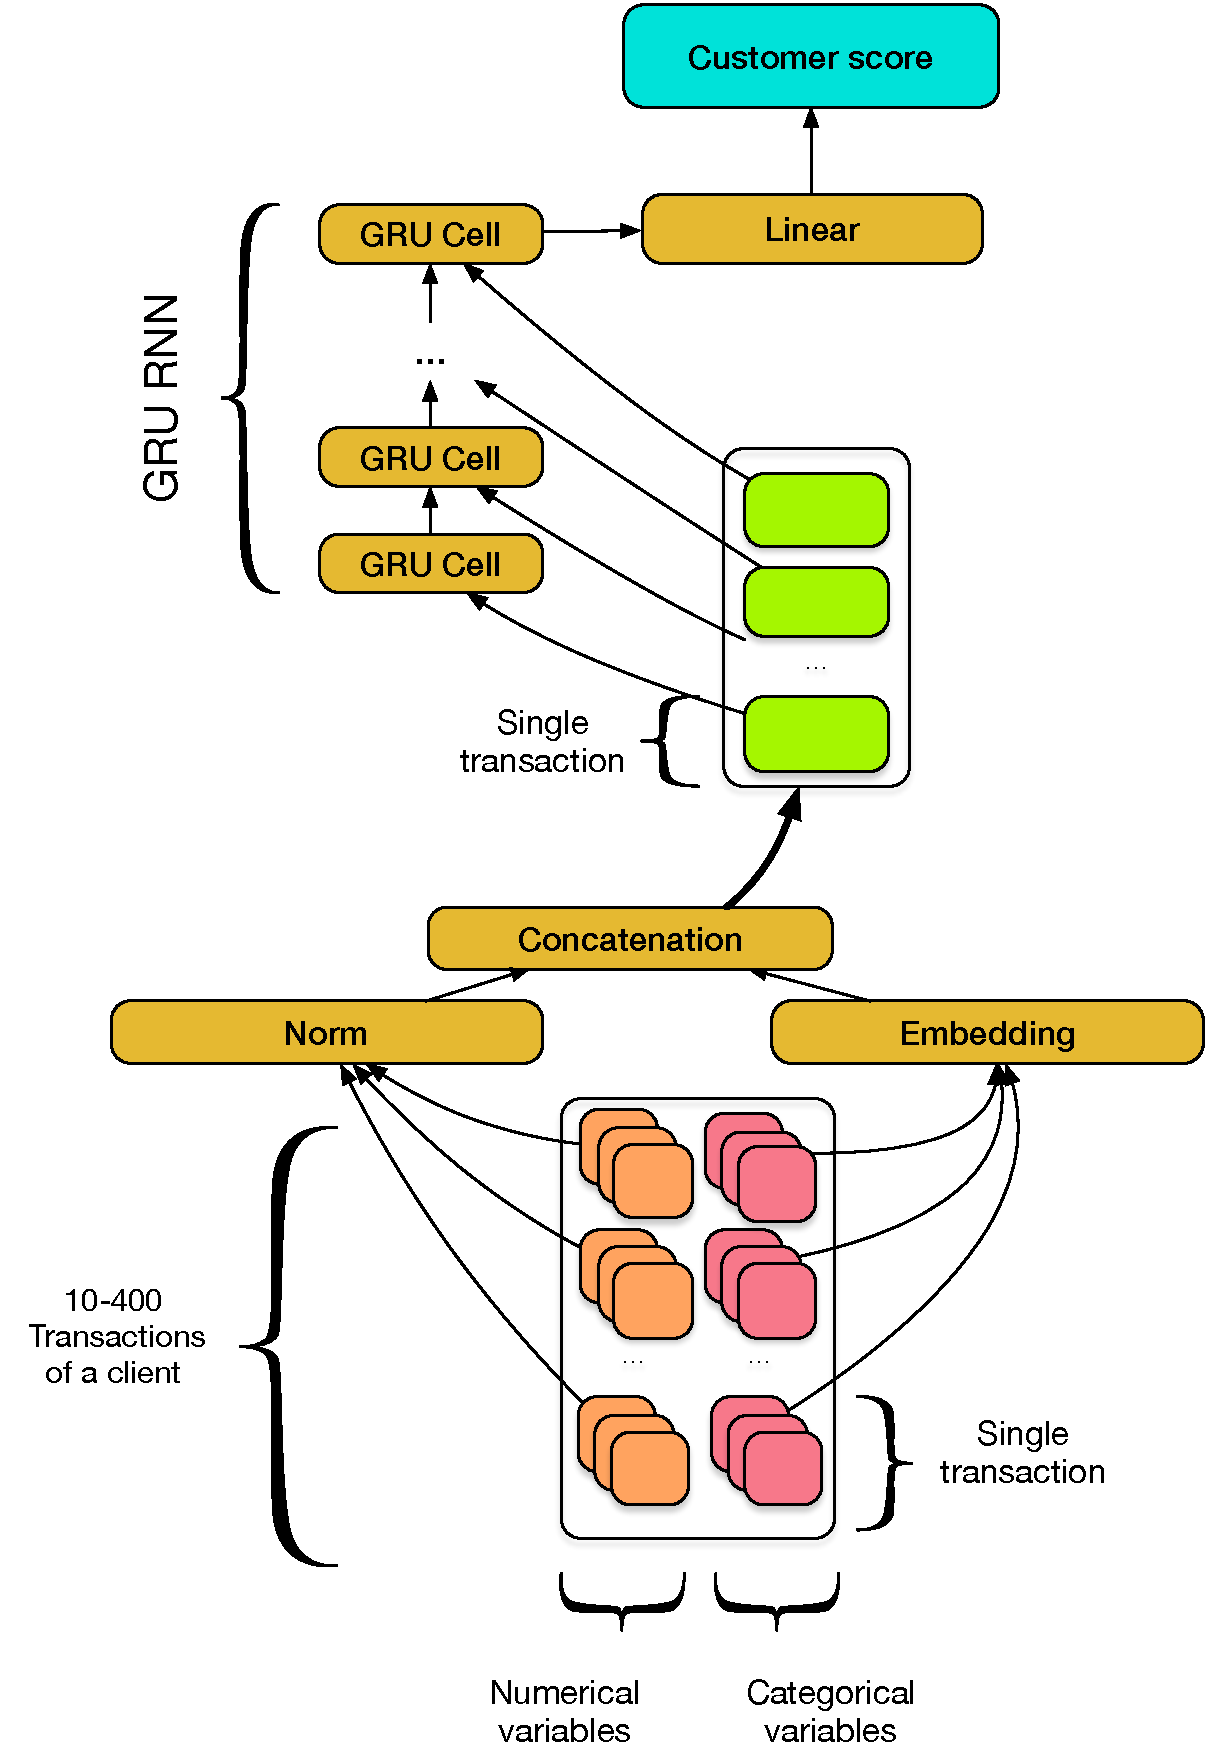
\includegraphics[width=0.46\textwidth]{architecture.pdf}
  \label{fig-arch}
\end{figure}


\subsection{Loss function}

To measure the quality of the scoring models it is possible to use different quantitative indexes such as Gini index, K-S statistics, Lift, Mahalanobis distance. 
In this work we use ROC AUC as a quality metric, which can be easily transformed into Gini index ($G = 2A_{ROC} - 1$) used as internal scoring quality metric in the bank. 

Several loss functions can be used as a proxy for the task of maximising ROC AUC. The classic binary cross-entry loss: $L_{CE}(p, y) = - \sum_i y_ilog(p_i)$ is the default choice.
The other possible approach is to use ranking loss: $ L_R(p_1, p_2, y) = \max(0, -y * (p_1 - p_2) + margin $ which directly optimizes ROC AUC.

For production version we used margin ranking loss with margin 0.01 which showed best results on the test data. 

\subsection{Ensembling}

Ensembling is a way to increase both quality of the model and its stability at the expense of time and computational power. In our case we have a relative abundance of the negative class samples and can use different subsamples of the negative class samples for training each model in the ensemble. 

For production we settled to use mean predictions of an ensemble of six separately trained models as a practical balance between prediction quality and execution time. For discussion of ensemble quality gain and other possible ensembling strategies please see section 4.3

\section{Experiments}
\subsection{Data}

The available transaction data falls into subcategories - transaction-level (timestamp, country, amount, MCC) and card-level (issuing branch, card type), card-level data is duplicated verbatim for each transaction related to the corresponding card.

Our training dataset represented 1.1 million of clients with $\sim400$ M total transactions. As a target variable we used the event of default for consumer loan during a year after its disbursement.

Due to the risk of data non-stationarity we have opted to use out-of-time validation strategy as in \cite{KVAMME2018207} instead of out-of-sample validation as used in \cite{khandani2010consumer} and \cite{bellotti2013forecasting}. Our results for out-of-fold validation were consistently higher than out-of-time validation for a range of architectures and hyperparameters.

We have used data for period Aug 2015 - Nov 2017 for training  (1 million of applications, 60 thousands of defaults) and period Dec 2017 - Mar 2017 for out-of-time validation (100 thousands of applications, 15 thousands of defaults).

Due to a large disparity between number of positive and negative cases we settled on the following sampling strategy: before each experiment we selected all positive cases and 10 times as much randomly selected negative cases, on each training epoch we used all positive cases and an equal number of negative cases, selected from the negative cases pool.

All models in this paper where trained on last 800 transactions for each customer, padding by zero was applied when the actual transaction count for a client was lower.

\subsection{Baselines}

To compare our model with other approaches to classification we have taken existing model which was used in bank for some time. For the thought comparison we also implemented additional model based on gradient boosting machine (Friedman\cite{friedman2001greedy} method.

Both Logistic regression  and Gradient boosting machine methods (Friedman\cite{friedman2001greedy}) was used as the classifier which gets large vector of hand-crafted aggregate features as an input. An example of aggregate feature would be the mean spends in some category of merchants (e. g. hotels).

We used LightGBM\cite{Ke2017LightGBMAH} implementation of GBM algorithm and created nearly 7000 aggregate features per sample. For current approach with lgistic regresion around 400 aggregate features was used. weight of evidence coding and binning of predictors was used for categorical features
\cite{lund2016woe}. 

\subsection{Offline execution of our method}

\subsubsection{Encoder architecture selection}

We experimented with different encoder architectures, but increasing number of layers, using Long Short Term Memory (LSTM) and using bidirectional recurrent cells did not improve on the quality of the model, the results are presented in Table 2

\begin{table}
\caption{Encoder architecture comparison}
\begin{tabular}{ | l | c |  }
\hline
& \textbf{validation ROC-AUC} \\
\hline
\textbf{GRU 1-layer} & 0,62  \\
\textbf{GRU 2-layer} & 0,67  \\
\textbf{LSTM 1-layer} & 0,67  \\
\textbf{LSTM 2-layer} & 0,67  \\
\textbf{GRU 1-layer Bidirectional} & 0,67  \\
\hline
\end{tabular}
\label{tab3}
\end{table}


\subsubsection{Latent space dimensionality}

The dimensionality of the embedding layers is an optimizable hyperparameter. It is worth noting that the total number of trainable weights in embedding layer is significantly higer than the number of weights in the encoder and decoder. We found that after reaching certain size further increase in number of latent space dimensions provided few if any benefits, see graph 1.

Graph: Ox-epoch, Oy-Train/Validation ROC-AUC , Series: (small, medium, big)

\subsubsection{Loss function and learning rate}

For all experiments we used a batch size of 32 for training and batch size of 768 for validation. When using ranking loss a new hyperparameter is introduced into the model - loss margin size. We found that margin size 0.01 gives best results among all the loss variants we tried, see table 3. 

\begin{table}
\caption{Loss comparison}
\begin{tabular}{ | l | c |  }
\hline
& \textbf{validation Gini} \\
\hline
\textbf{BCE Loss} & 0,62  \\
\textbf{Hinge loss 0.5} & 0,67  \\
\textbf{Hinge loss 0.1} & 0,67  \\
\textbf{Hinge loss 0.01} & 0,67  \\
\textbf{Hinge loss 0.01 + BCE Loss} & 0,67  \\
\hline
\end{tabular}
\label{tab4}
\end{table}

Learning rate and learning rate reduction schedule is one of the most sensitive hyper-parameters which can dramatically change the performance of the model.
We found that optimal learning rate schedule depends heavily on loss function used, batch size and overall number of parameters in the model. 
We tried several learning rates and several learning rate reduction regimes. We found that for both BCE loss and ranking loss the most effective strategy was an aggressive linear learning rate reduction with gamma=0.5, see graph 2.

Graph: Ox-epoch, Oy-Train/Validation ROC AUC , Series: (lr=0.0001 const, lr decreasing g=0.8, g=0.5, cyclical g =0.5) 

\subsubsection{Regularization methods}

Due to the low number of positive classes all models exhibit a propensity for ovefitting, therefore we tried various types of dropout regularisation:
\begin{itemize}
\item Transaction dropout - randomly remove a share of client transactions
\item Transaction shuffle - randomly permute the order of client transactions
\item Transaction concatenation - create synthetic training examples by concatenation of transaction histories for two clients from the same class
\item Embedding dropout - randomly zero some components after embedding layer
\item Encoder dropout - randomly zero some components after encoder
\end{itemize}
None of the mentioned regularization methods proved effective against overfitting, see graph 3.

Graph: Ox-epoch, Oy-Train/Validation Gini , Series: (baseline, trx do, emb do, emb shuffle,)

\subsubsection{Ensembling methods}

Averaging the predictions of different models trained with distinct negative class examples leads to both increased accuracy and reduced variabilty of results, see Box-plot 1

Box-plot: Series = {Single, Ens-3, Ens-6  diff loss? } Cols = {val ROC AUC + STD}
best hyperparams

Another ensembling method is Stochastic Weight averaging (SWA) proposed by Izmailov et al.\cite{DBLP:journals/corr/LoshchilovH16a} This approach can significantly reduce inference time since only one model with averaged weights is used instead of the whole ensemble. But in our case averaging of weights of different models led to significant reduction in quality.

Yet another approach is to use snapshots of the same model in the final ensemble as proposed by Huang et al.\cite{DBLP:journals/corr/HuangLPLHW17} It can significantly reduce training time since only one model should be trained.

We found that combining SWA with snapshot ensembling for single model training by taking snapshots after a set epoch and averaging the weights leads to some reduction of variability, but the results were inconclusive and we opted for not using these advanced ensembling methods in our production model.


\subsection{Moving to production}

We performed massive field test of our neural scoring model in bank's production pipeline. We used the model trained on the datased discussed
The model was used to make decision about credit application for tens of thousands of applicants during one month (Dec 2018).
The preliminary financial results are measured in tens of millions of dollars per year which is very significant result for the bank of this type and size.

\section{Results}
\begin{table}
\caption{Experiment comparison}
\begin{tabular}{ | p{12em} | c | c | }
\hline
& \textbf{ROC AUC} & \textbf{N Features} \\
\hline
\textbf{Logistic regression on aggregate features} & 0.78 & $\sim400$ \\
\textbf{LGBM on aggregate features} & 0.81 & $\sim7000$ \\
\textbf{RNN on detailed data} & 0.84 & 16 \\
\hline
\end{tabular}
\label{tab2}
\end{table}

The comparison of validation results can be seen in Table \ref{tab2}. Training and validation sets were the same for each model.  As you can see RNN can significantly outperform classical ML approaches with hand-crafted features given enough data.

\begin{figure}
  \caption{RNN has steeper learning curve than LGBM.}
  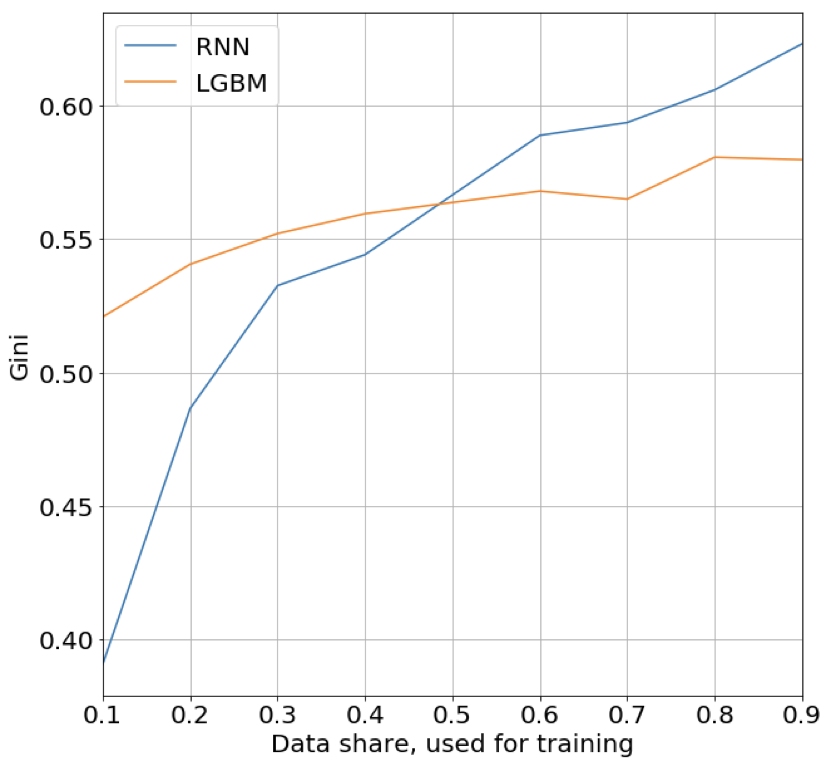
\includegraphics[width=0.46\textwidth]{learning-curve.png}
  \label{fig-lc}
\end{figure}

On \ref{fig-lc} there is the learning curve for RNN and LGBM models. As you can see for the small number of training samples LGBM with hand-crafted features is better than RNN but if we have enough data RNN can perform significantly better. Also, RNN has steeper learning curve than LightGBM hence the performance gap would increase with more data.

\subsection{Minimal number of training samples}

The main limitation of our method is availability of enough training examples of default applications. As you can see on \ref{fig-lc} around 15 thousands facts of default is required for to make neural net model which i
 better than gradient boosting machine model.

\subsection{Transaction count}

\begin{figure}
  \caption{Around 100 transactions is enough for confident classification}
  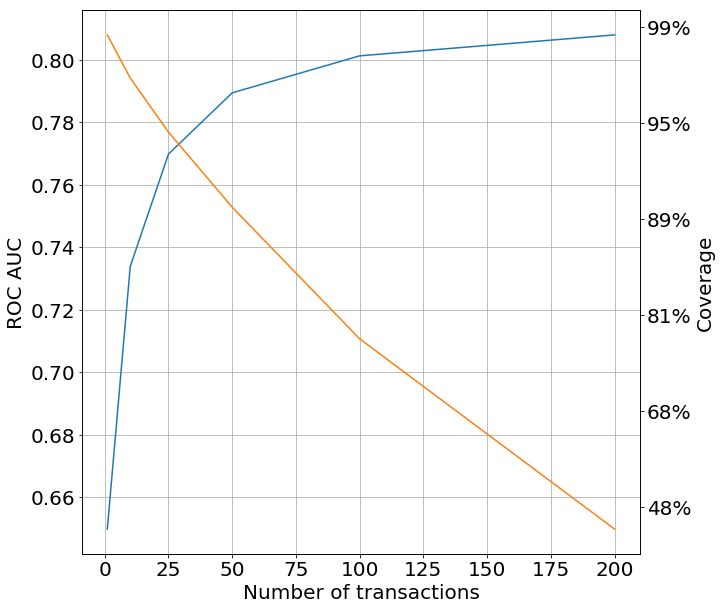
\includegraphics[width=0.46\textwidth]{information-vs-accuracy.png}
  \label{fig-tc}
\end{figure}

One of the limitations of our method is the minimum number of transaction per client. We can see on figure\ref{fig-tc} that nearly one hundred of transactions is desirable to confidently estimate the default probability of a client. Regarding our dataset, half of the bank clients with plastic card have more than one hundred transactions.

\subsection{Discussion}

While interpretation of the black-box model like LSTM or GRU is exceptionally hard, it is possible to change the architecture of the network to make it interpretable without sacrificing significant part of its classification quality.

One of such changes was proposed by Choi et al.\cite{DBLP:journals/corr/ChoiBSSS16} by the name of RETAIN. The idea is that RNN is not used to perform encoding of the multivariate time-series but instead generates attention weights for each input vector. Then that weights are used to calculate linear combination of input vectors which is finally used for classification.

It is possible to calculate contribution of each input vector to the final prediction. It is possible to apply RETAIN or similar approach to change the architecture of our model.

\section{Conclusions}

Neural network based model is hungry for data but can outperform classical ML approaches. The other huge advantage of the neural net based approach is unsupervised feature learning. There is almost no need to manually design features which saves tons of time for the data scientist.

+ Regularization 

The main disadvantage of the neural net based approach is its black-box nature. However, this is the active topic of the research. Some approaches to interpretation like RETAIN can already shed some light to the inner logic of the model.

+ Contributions

\subsection{Future work}

One of the approach to overcome this limitation would be use of the transfer learning techniques. We have done some preliminary research where we tried to create a scoring model for mortgage loans instead of retail credits. We used trained neural network for model retail credits as a start and then fine-tuned it using additional training samples for mortgage loans. As you can see in table the fine-tuned model has shown significantly better performance than the model built only on mortgage loans data.

\bibliographystyle{abbrv}
\bibliography{sigproc}

\end{document}
